\documentclass[12pt,t]{beamer}

%------------------------------------------------------------------------------
% configuration
%------------------------------------------------------------------------------
\RequirePackage{etex}
\usepackage{../../themes/dbt}
\usepackage{catchfilebetweentags}

\setbeameroption{hide notes}

\graphicspath{{images/}}

% a few macros
\newcommand{\bi}{\begin{itemize}}
\newcommand{\ei}{\end{itemize}}
\newcommand{\ig}{\includegraphics}
\newcommand{\myhref}[1]{\href{#1}{\tt \scriptsize #1}}
\newcommand{\incnote}[1]{\note{\ExecuteMetaData[notes.tex]{#1}}}

%------------------------------------------------------------------------------
% title
%------------------------------------------------------------------------------
% slide
\title{Systèmes d'exploitation pour l'embarqué}
\subtitle{UV 5.2 - Exécution et Concurrence}

\author{\href{}{Paul Blottière}}
\institute{
    \href{http://www.ensta-bretagne.fr/}{ENSTA Bretagne} \\[2pt]
    \href{}{\tt \scriptsize 10 Novembre 2015}
}
\date{
    \href{https://github.com/pblottiere}{\tt \scriptsize https://github.com/pblottiere}
}

% info
\begin{document}

{
\setbeamertemplate{footline}{} % no page number here
\frame{
    \titlepage
    \incnote{title}
} }

%------------------------------------------------------------------------------
% amélioration continue
%------------------------------------------------------------------------------
\begin{frame}{Amélioration continue}
    \subt{Contributions}
    \vspace{12pt}

    \begin{center}
    
\includegraphics[scale=0.7]{github.png}
    \end{center}

    \bi
    \itemsep12pt
    \item Dépôt du cours : \href{https://github.com/pblottiere/embsys}{\tt \scriptsize https://github.com/pblottiere/embsys}
    \item Souhaits d'amélioration, erreurs, ... : ouverture d'issues (avec le bon tag!)
    \item Apports de correction : Pull Request
    \ei
\end{frame}

%------------------------------------------------------------------------------
% organisation
%------------------------------------------------------------------------------
\begin{frame}{Organisation}
    \vspace{12pt}

    \bi
        \itemsep12pt
        \item 9 CM
        \item 6 TE
        \item 2 BE
    \ei

    \incnote{organisation}
\end{frame}

%------------------------------------------------------------------------------
% plan
%------------------------------------------------------------------------------
\begin{frame}{Plan}
    \subt{}

    \bi
        \itemsep6pt
        \item Un peu d'histoire
        \item Les normes
        \item Logiciel Libre et Logiciel Open-Source
        \item Licences de distribution
        \item Définitions et propriétés
        \item Architectures matérielles
        \item Quelques chiffres
        \item Les OS embarqués existant
        \item Comment choisir?
        \item Et si on choisit Linux?
    \ei

    \note {
    }
\end{frame}

%------------------------------------------------------------------------------
% histoire1
%------------------------------------------------------------------------------
\begin{frame}{Un peu d'histoire}
    \subt{Le premier jeu vidéo}
    \vspace{20pt}

    \begin{columns}[onlytextwidth]
        \begin{column}{0.45\textwidth}
            \centering
            1964 : Multics \\
            \vspace{30pt}
            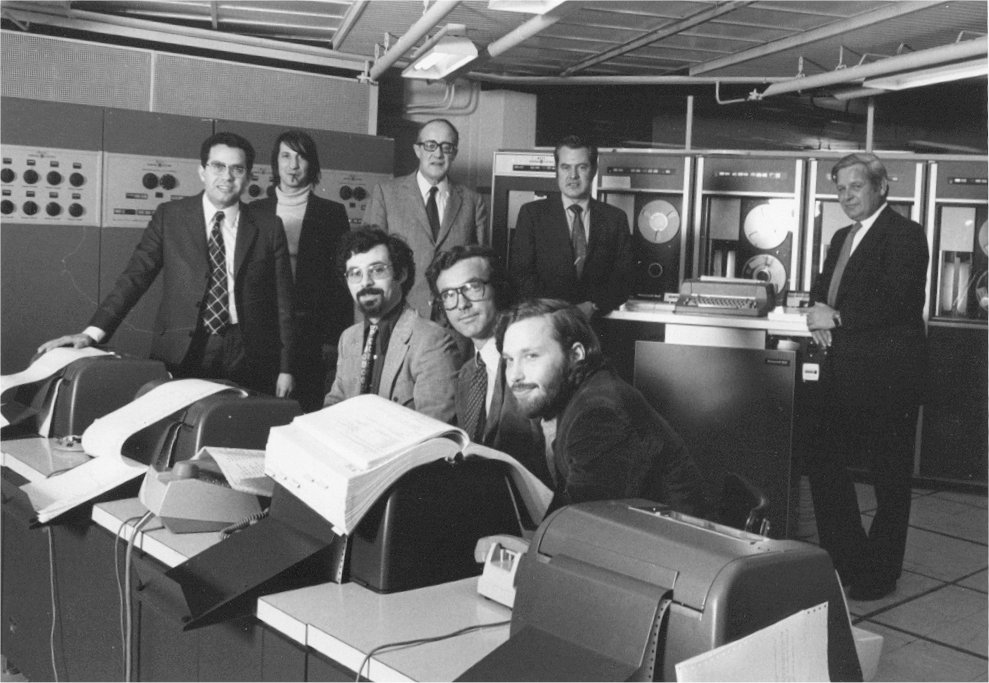
\includegraphics[scale=0.15]{ge645-paris.jpg}
        \end{column}
        \begin{column}{0.45\textwidth}
            \centering
            1969 : Space Travel/Unics par Ken Thompson \\
            \vspace{10pt}
            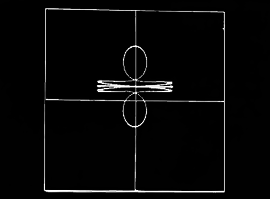
\includegraphics[scale=0.6]{space-travel.png}
        \end{column}
    \end{columns}

    \incnote{histoire1}
\end{frame}

%------------------------------------------------------------------------------
% histoire2
%------------------------------------------------------------------------------
\begin{frame}{Un peu d'histoire}
    \subt{La naissance du langage C}
    \vspace{30pt}

    \begin{columns}[onlytextwidth]
        \begin{column}{0.45\textwidth}
            \centering
            1971 : Le C par Dennis Ritchie \\
            \vspace{20pt}
            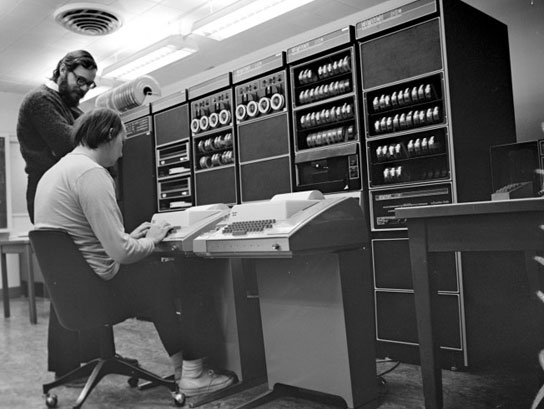
\includegraphics[scale=0.3]{ken-ritchie-1972.jpg}
        \end{column}
        \begin{column}{0.45\textwidth}
            \centering
            1983 : GNU par Stallman \\
            \vspace{20pt}
            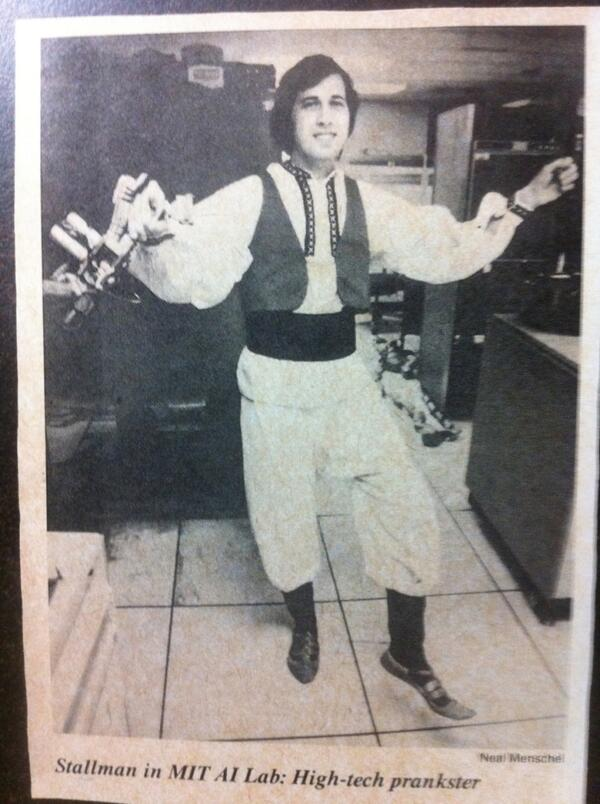
\includegraphics[scale=0.15]{rms-mitlab.jpg}
        \end{column}
    \end{columns}

    \incnote{histoire2}
\end{frame}

%------------------------------------------------------------------------------
% histoire3
%------------------------------------------------------------------------------
\begin{frame}{Un peu d'histoire}
    \subt{Un hobby devenu célèbre}
    \vspace{30pt}

    \begin{columns}[onlytextwidth]
        \begin{column}{0.45\textwidth}
            \centering
            1987 : Linux par Linus Torvalds \\
            \vspace{20pt}
            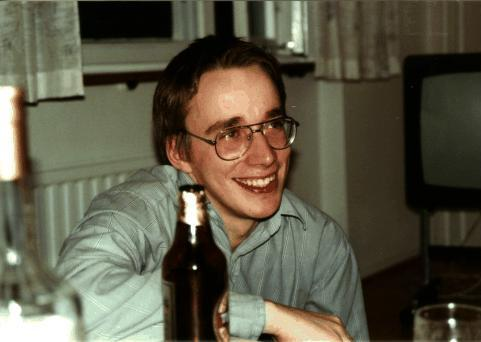
\includegraphics[scale=0.3]{linus.jpg}
        \end{column}
        \begin{column}{0.45\textwidth}
            \centering
            1992 : GNU / Linux \\
            \vspace{30pt}
            
\includegraphics[scale=0.2]{gnu-linux.png}
        \end{column}
    \end{columns}

    \incnote{histoire3}
\end{frame}

%------------------------------------------------------------------------------
% histoire4
%------------------------------------------------------------------------------
\begin{frame}{Un peu d'histoire}
    \subt{De nos jours}
    \vspace{5pt}

    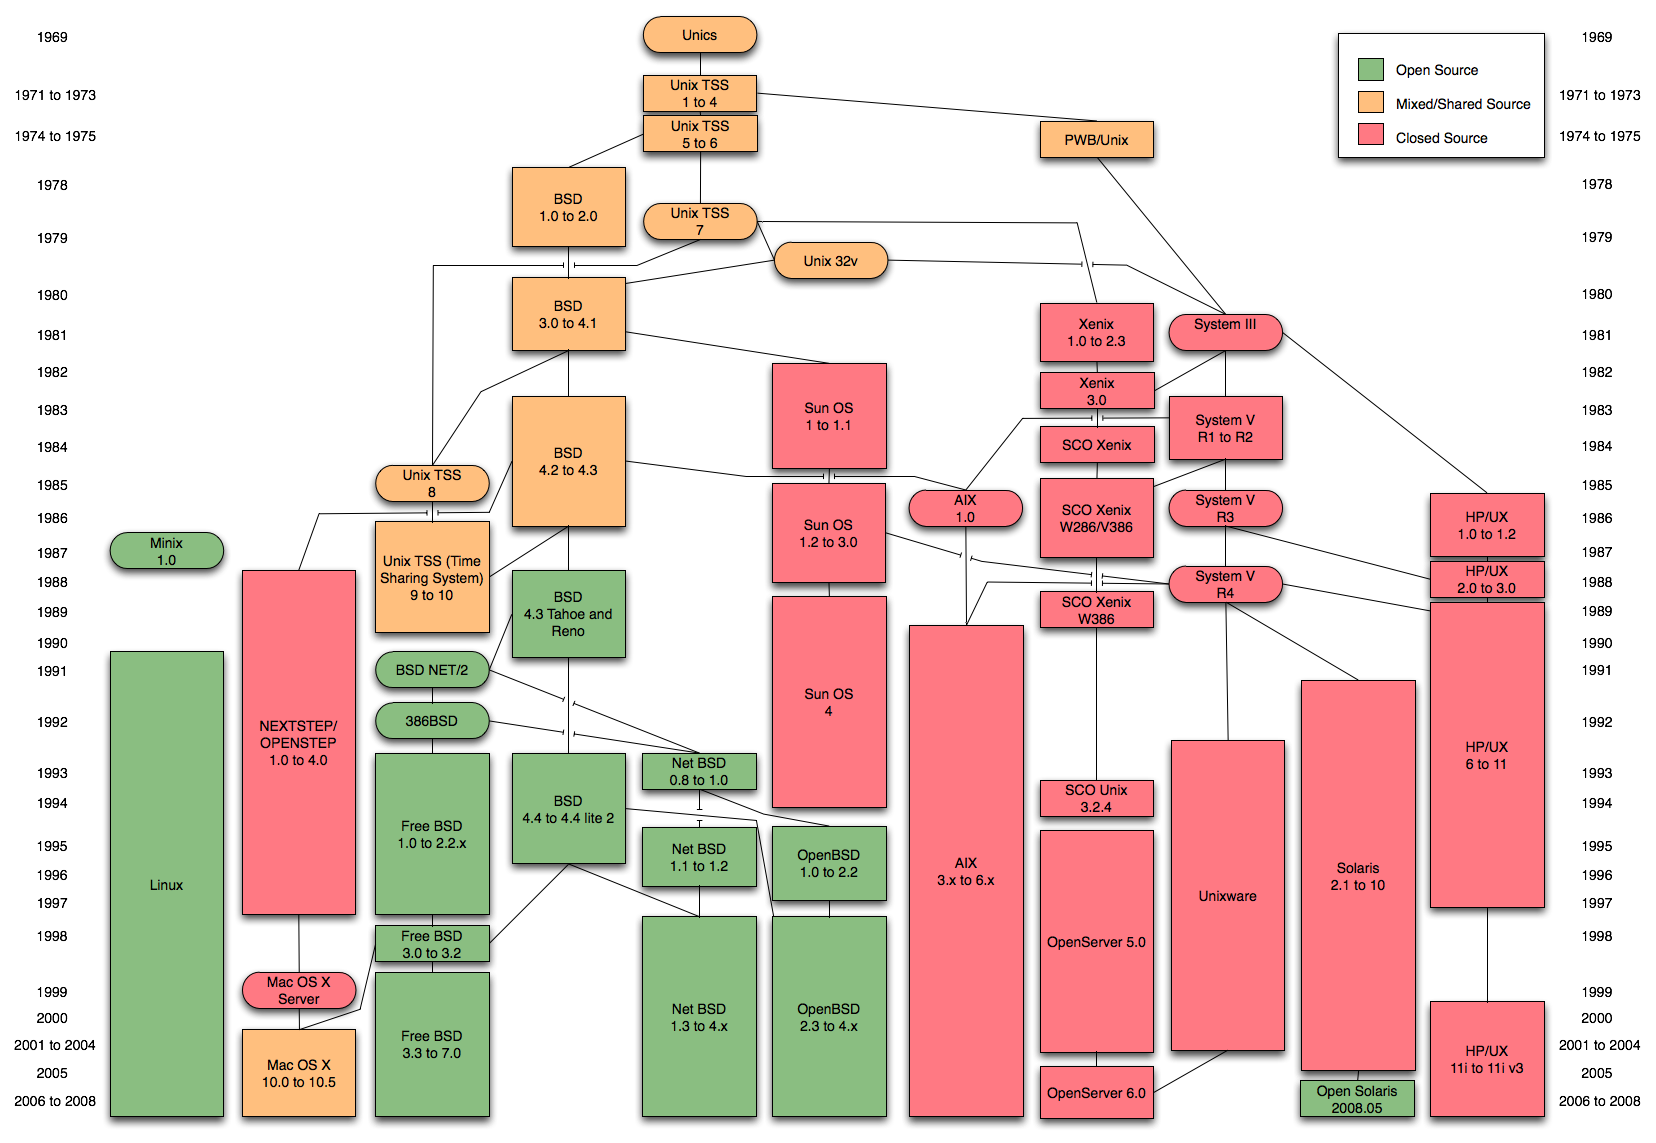
\includegraphics[scale=0.18]{timeline.png}

    \incnote{histoire4}
\end{frame}

%------------------------------------------------------------------------------
% normes1
%------------------------------------------------------------------------------
\begin{frame}{Les normes}
    \subt{SUSv3}
    \vspace{20pt}

    Des normes sont nécessaires pour assurer une compatibilité des logiciels
    entre systèmes d'exploitation:
    \vspace{10pt}
    \bi
    \itemsep12pt
    \item 1988 : Portable Operating System Interface (POSIX). Plusieurs versions : 1,
                 1.b, 1.c
      \item 1997 : UNIX98 ou Single UNIX Specification V2
    \item Standard actuel : SUS V3 (fusion entre POSIX et UNIX98)
    \ei

    \vspace{10pt}
    \centering
    \myhref{http://www.unix.org/version3/}

    \incnote{normes1}
\end{frame}

%------------------------------------------------------------------------------
% normes2
%------------------------------------------------------------------------------
\begin{frame}[fragile]{Les normes}
    \subt{POSIXLY\_CORRECT SIR!}
    \vspace{10pt}

    POSIX:
    \begin{lstlisting}[language=bash]
    tool [-a][-b][-c option_argument] \
        [-d|-e][-f[option_argument]][operand...]
    \end{lstlisting}

    \vspace{10pt}
    Sous GNU/Linux, les règles sont différentes!

    \vspace{10pt}
    Conséquences sous une distribution Linux:

    \begin{lstlisting}
    > ls -a .
    .vimrc .vim devel doc
    > ls . -a
    .vimrc .vim devel doc
    > POSIXLY_CORRECT=1 ls . -a
    ls: impossible d'accéder à -a: Aucun fichier ou
        dossier de ce type
    .vimrc .vim devel doc
    \end{lstlisting}

    \incnote{normes2}
\end{frame}

%------------------------------------------------------------------------------
% opensource1
%------------------------------------------------------------------------------
\begin{frame}{Logiciel Libre et Logiciel Open Source}
    \subt{Question de philosophie...}
    \vspace{20pt}

    \bi
    \item Logiciel Libre : code source ouvert et pouvant être modifié. Fond
        philosophique => liberté des utilisateurs (Free as Freedom)!
    \vspace{20pt}
    \item Logiciel Open Source : code source ouvert et pouvant être modifié...
          Fond pragmatique => efficacité, praticité!
    \ei

    \vspace{10pt}

    \centering
    \myhref{http://www.gnu.org/philosophy/free-software-for-freedom.fr.html}

    \incnote {opensource1}
\end{frame}

%------------------------------------------------------------------------------
% opensource2
%------------------------------------------------------------------------------
\begin{frame}{Logiciel Libre et Logiciel Open Source}
    \subt{Origine des licences GPL et LGPL}
    \vspace{15pt}

    \vspace{5pt}
    \begin{center}
    1985 \\
    \vspace{10pt}
    
\includegraphics[scale=0.5]{fsf.png}
    \end{center}
    \vspace{5pt}

    Son but:
    \bi
    \itemsep12pt
    \item protéger les utilisateurs contre les logiciels "privateurs"
    \item élaborer des licences de distribution
    \ei

    \incnote{opensource2}
\end{frame}

%------------------------------------------------------------------------------
% licences1
%------------------------------------------------------------------------------
\begin{frame}{Licences de distribution}
    \subt{Copyleft}
    \vspace{20pt}

    L'utilisateur refuse qu'une évolution quelconque de son travail soit
    accompagnée d'une restriction!

    \vspace{40pt}
    \centering
    
\includegraphics[scale=0.25]{copyleft.png}

    \incnote {licences1}
\end{frame}

%------------------------------------------------------------------------------
% licences2
%------------------------------------------------------------------------------
\begin{frame}{Licences de distribution}
    \subt{GPL et LGPL}
    \vspace{20pt}

    Licence libre copyleft :
    \bi
    \item GPL : GNU General Public Licence. Édition de liens possible qu'avec du
          code GPL! \myhref{http://www.gnu.org/licenses/gpl-3.0.fr.html}
      \item LGPL : Lesser GPL. Édition de liens moins restrictive! \myhref{http://www.gnu.org/licenses/lgpl-3.0.fr.html}
    \ei

    \vspace{20pt}
    Licence libre non copyleft :
    \bi
    \item BSD : les versions modifiées ne sont elles mêmes pas nécessairement
          libres!
    \item ...
    \ei

    \incnote {licences2}
\end{frame}

%------------------------------------------------------------------------------
% licences3
%------------------------------------------------------------------------------
\begin{frame}[fragile]{Licences de distribution}
    \subt{Conséquences dans la vie courante...}
    \vspace{15pt}

    Examples de licences:
    \bi
    \itemsep6pt
    \item nmap : GPL {\tt /usr/share/doc/nmap/copyright}
    \item GNU C library : LGPL {\tt /usr/share/doc/libc6/copyright}
    \ei
    \vspace{20pt}

    Debian et le DFSG (Debian Free Software Guideline) :
    \bi
    \item {\tt main} : paquets conforme au DFSG
    \item {\tt contrib} : paquets conforme au DFSG mais avec des dépendances en
        dehors du {\tt main}
    \item {\tt non-free} : paquets non conforme au DFSG
    \ei

    \incnote{licences3}
\end{frame}

%------------------------------------------------------------------------------
% licences4
%------------------------------------------------------------------------------
\begin{frame}[fragile]{Licences de distribution}
    \subt{Conséquences dans la vie courante...}
    \vspace{20pt}

    VRMS (Virtual RMS) :
    \vspace{15pt}
    \begin{lstlisting}
> vrms
Contrib packages installed on multi
flashplugin-nonfree            Adobe Flash Player
1 contrib packages, 0.0% of 2877 installed packages
    \end{lstlisting}

\end{frame}

%------------------------------------------------------------------------------
% def1
%------------------------------------------------------------------------------
\begin{frame}{Définitions et propriétés}
    \subt{Kernel et système d'exploitation}
    \vspace{10pt}

    Kernel :
    \bi
    \item noyau d'un système d'exploitation
    \item gère les ressources matérielles
    \item permet la communication entre composants logiciels/matériels
    \item existe plusieurs architectures (voir cours suivant)
    \ei

    \vspace{10pt}
    Système d'exploitation:
    \bi
    \item kernel + logiciels comme compilateur, shell, debuger, ...
    \item couche d'abstraction par rapport au matériel
    \item interface générique de programmation
    \ei

    \incnote{def1}
\end{frame}

%------------------------------------------------------------------------------
% def2
%------------------------------------------------------------------------------
\begin{frame}{Définitions et propriétés}
    \subt{Dans le monde des systèmes embarqués...}
    \vspace{5pt}

    Système embarqué:
    \bi
    \itemsep4pt
    \item composition d'une partie électronique et logicielle
    \item souvent très limitée d'un point de vue ressources matérielles (CPU,
          mémoire, ...)
    \item autonome, durée de vie très longue (plus de 20ans pour les systèmes
          militaires)
    \item doit respecter des contraintes d'environnement (vibration, chaleur,
          ...)
    \ei

    \vspace{5pt}
    \centering
    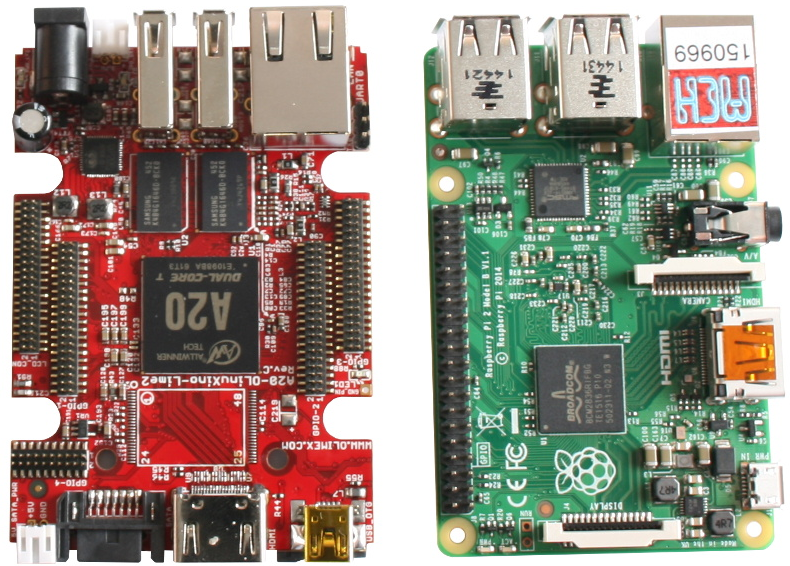
\includegraphics[scale=0.13]{ol-rasp.png}

    \incnote{def2}
\end{frame}

%------------------------------------------------------------------------------
% def3
%------------------------------------------------------------------------------
\begin{frame}{Définitions et propriétés}
    \subt{Dans le monde des systèmes embarqués}
    \vspace{20pt}

    Système d'exploitation embarqué:
    \bi
    \itemsep6pt
    \item OS sur lequel un logiciel embarqué va être exécuté.
    \item Contrainte forte par rapport à la consommation matérielle /
          énergétique.
    \item OS classique souvent inenvisageable
    \ei
    \vspace{10pt}

    Système d'exploitation temps réel (vs temps partagé):
    \bi
    \itemsep6pt
    \item garantit les temps de réponse (temps réel dur/mou, préemptivité du
          Kernel, ...)
    \item Voir le cours associé!
    \ei

    \incnote{def3}
\end{frame}

%------------------------------------------------------------------------------
% def4
%------------------------------------------------------------------------------
\begin{frame}{Définitions et propriétés}
    \subt{Dans le monde des systèmes embarqués}
    \vspace{10pt}

    Logiciel embarqué:
    \bi
    \itemsep6pt
    \item logiciel intégré pour une application dédiée
    \item un bon logiciel embarqué est un logiciel dont on oubli l'existence!
    \ei

    \vspace{10pt}
    Linux embarqué
    \bi
    \itemsep6pt
    \item Kernel Linux + composants open-source
    \item construit sur mesure par rapport aux besoins
    \ei

    \vspace{10pt}
    \centering
    
\includegraphics[scale=0.8]{linux-embedded.png}

    \incnote{def4}
\end{frame}

%------------------------------------------------------------------------------
% def5
%------------------------------------------------------------------------------
\begin{frame}{Définitions et propriétés}
    \subt{Rappels : microcontrôlleur vs microprocesseur}
    \vspace{10pt}

    Microprocesseur:
    \bi
    \itemsep6pt
    \item séquenceur
    \item unité arithmétique et logique (UAL)
    \item registre
    \item unité d'entrée sortie (analogique)
    \ei

    \vspace{10pt}
    Microcontrôlleur:
    \bi
    \itemsep6pt
    \item microprocesseur peu puissant (fréquence d'horloge faible, largeur des
          registres restreinte : 4 bits/8bits contre 32 bits/64bits, ...)
    \item mémoire intégrée
    \item entrées/sorties analogiques et numériques
    \ei

    \incnote{def4}
\end{frame}

%------------------------------------------------------------------------------
% chiffres1
%------------------------------------------------------------------------------
\begin{frame}{Quelques chiffres}
    \subt{Les systèmes embarqués sont partout!}
    \incnote{chiffres1}
\end{frame}

%------------------------------------------------------------------------------
% chiffres2
%------------------------------------------------------------------------------
\begin{frame}{Quelques chiffres}
    \subt{Soutien des états}
    \incnote{chiffres2}
\end{frame}

%------------------------------------------------------------------------------
% chiffres3
%------------------------------------------------------------------------------
\begin{frame}{Quelques chiffres}
    \subt{Répartition du Chiffre d'Affaires}
    \incnote{chiffres3}
\end{frame}

%------------------------------------------------------------------------------
% chiffres4
%------------------------------------------------------------------------------
\begin{frame}{Quelques chiffres}
    \subt{Répartition des effectifs}
    \incnote{chiffres4}
\end{frame}

%------------------------------------------------------------------------------
% embos1
%------------------------------------------------------------------------------
\begin{frame}{Les OS embarqués existant}
    \subt{Sans base Linux}
    \incnote{embos1}
\end{frame}

%------------------------------------------------------------------------------
% embos2
%------------------------------------------------------------------------------
\begin{frame}{Les OS embarqués existant}
    \subt{A base de Linux}
    \incnote{embos2}
\end{frame}

%------------------------------------------------------------------------------
% choice1
%------------------------------------------------------------------------------
\begin{frame}{Comment choisir?!}
    \subt{Systèmes propriétaires ?}
    \incnote{choice1}
\end{frame}

%------------------------------------------------------------------------------
% choice2
%------------------------------------------------------------------------------
\begin{frame}{Comment choisir?}
    \subt{Systèmes Open Source?}
    \incnote{choice2}
\end{frame}

%------------------------------------------------------------------------------
% linux1
%------------------------------------------------------------------------------
\begin{frame}{Et si on choisit Linux...}
    \subt{Avantages}
    \incnote{linux1}
\end{frame}

%------------------------------------------------------------------------------
% linux2
%------------------------------------------------------------------------------
\begin{frame}{Et si on choisit Linux...}
    \subt{Avantages}
    \incnote{linux2}
\end{frame}

%------------------------------------------------------------------------------
% linux3
%------------------------------------------------------------------------------
\begin{frame}{Et si on choisit Linux...}
    \subt{Inconvénients}
    \incnote{linux3}
\end{frame}

%------------------------------------------------------------------------------
% hard1
%------------------------------------------------------------------------------
\begin{frame}{Aspect matériel}
    \subt{Processeurs}
    \incnote{hard1}
\end{frame}

%------------------------------------------------------------------------------
% hard2
%------------------------------------------------------------------------------
\begin{frame}{Aspect matériel}
    \subt{MMU}
    \incnote{hard2}
\end{frame}

%------------------------------------------------------------------------------
% ref
%------------------------------------------------------------------------------
\begin{frame}{Références}

\end{frame}

\end{document}
